%!TEX root = ../../../main.tex

\subsection{Experimental results on MuHAVi dataset}
    \paragraph{1) Cross-view validation:} Table.\ref{tab:muhavi_cross} illustrates cross-view recognition results. The proposed pc-MvDA consistently produces a better average accuracy of around 96.19\% for protocol 1, approximately 4.55\% and 1.51\% higher than that of MvDA (91.64\%) and MvDA-vc (94.67\%) respectively.

    \begin{table}[htbp]
    \centering
    \caption{Cross-view recognition comparison on MuHAVi dataset}
    \resizebox{0.8\textwidth}{!}{
    \begin{tabular}{|c|c|c|c|c|c|c|}
        \hline
        \multirow{2}{*}{Deep features}          & \multicolumn{3}{c|}{Protocol 1}   & \multicolumn{3}{c|}{Protocol 2}           \\ \cline{2-7} 
                                                & MvDA  & MvDA-vc & pc-MvDA         & MvDA  & MvDA-vc        & pc-MvDA          \\ \hline
        \multicolumn{1}{|c|}{C3D}               & 92.85 & 95.15   & \textbf{97.65}  & 98.95 & 99.76          & \textbf{100}     \\ \hline
        \multicolumn{1}{|c|}{ResNet-50 3D}      & 97.94 & 99.15   & \textbf{99.18}  & 96.77 & \textbf{99.94} & \textbf{99.94}   \\ \hline
        \multicolumn{1}{|c|}{ResNet-50 RNN}     & 95.54 & 95.14   & \textbf{96.18}  & 98.70 & 99.05          & \textbf{99.99}   \\ \hline
        \multicolumn{1}{|c|}{ResNet-50 TA}      & 85.80 & 88.95   & \textbf{91.12}  & 96.57 & 97.03          & \textbf{99.88}   \\ \hline
        \multicolumn{1}{|c|}{ResNet-50 AP}      & 86.09 & 94.98   & \textbf{96.82}  & 89.04 & 98.62          & \textbf{99.93}   \\ \hline
    \end{tabular}}
    \label{tab:muhavi_cross}
    \end{table}

    %Results in Table.\ref{tab:cross_feature_muhavi} show that our combination with ResNet-50 3D has the highest accuracies in almost every circumstances, even though both features coupled with our proposed pc-MvDA give satisfactory performance with all scores exceeding 91\%.

    \begin{table}[htbp]
    \centering
    \caption{Cross-view recognition results of different features on MuHAVi dataset with pc-MvDA method. The result in the bracket are accuracies of using features C3D, ResNet-50 3D, ResNet-50 RNN, ResNet-50 TA, ResNet-50 AP respectively. Each row corresponds to training view (from view C1 to view C7). Each column corresponds to testing view (from view C1 to view C7)}
    \resizebox{\textwidth}{!}{\begin{tabular}{|c|c|c|c|c|c|c|c|}
        \hline
        \backslashbox{Training}{Testing} & C1 & C2 & C3 & C4 & C5 & C6 & C7 \\ \hline
        C1 & N/A & \begin{tabular}{@{}c@{}} (96.1, \textbf{100}, 96.8, \\ 88.5, 98.5) \end{tabular} & \begin{tabular}{@{}c@{}} (98.6, \textbf{99.6}, 96.6, \\ 88.9, 96.3) \end{tabular} & \begin{tabular}{@{}c@{}} (98.6, \textbf{99.6}, 98.0, \\ 93.1, 98.2) \end{tabular} & \begin{tabular}{@{}c@{}} (97.7, \textbf{99.6}, 95.4, \\ 91.3, 96.1) \end{tabular} & \begin{tabular}{@{}c@{}} (97.7, \textbf{98.4}, 92.3, \\ 93.1, 96.3) \end{tabular} & \begin{tabular}{@{}c@{}} (98.2, \textbf{98.5}, 97.2, \\ 89.8, 97.1) \end{tabular} \\ \hline
        C2 & \begin{tabular}{@{}c@{}} (95.6, \textbf{99.0}, 95.2, \\ 91.3, 95.5) \end{tabular} & N/A & \begin{tabular}{@{}c@{}} (98.9, \textbf{99.6}, 96.9, \\ 90.3, 96.1) \end{tabular} & \begin{tabular}{@{}c@{}} (98.4, \textbf{99.6}, 97.6, \\ 92.6, 98.2) \end{tabular} & \begin{tabular}{@{}c@{}} (97.7, \textbf{99.6}, 95.4, \\ 90.9, 96.1) \end{tabular} & \begin{tabular}{@{}c@{}} (97.8, \textbf{98.4}, 92.7, \\ 93.6, 96.5) \end{tabular} & \begin{tabular}{@{}c@{}} (98.6, \textbf{99.0}, 97.4, \\ 90.6, 96.9) \end{tabular} \\ \hline
        C3 & \begin{tabular}{@{}c@{}} (96.1, \textbf{99.0}, 95.6, \\ 90.3, 95.1) \end{tabular} & \begin{tabular}{@{}c@{}} (97.0, \textbf{100}, 96.7, \\ 88.4, 97.8) \end{tabular} & N/A & \begin{tabular}{@{}c@{}} (98.1, \textbf{99.2}, 98.2, \\ 92.8, 98.2) \end{tabular} & \begin{tabular}{@{}c@{}} (97.9, \textbf{99.6}, 95.4, \\ 90.2, 95.6) \end{tabular} & \begin{tabular}{@{}c@{}} (97.9, \textbf{98.2}, 93.0, \\ 94.2, 96.5) \end{tabular} & \begin{tabular}{@{}c@{}} (97.8, \textbf{98.7}, 97.4, \\ 89.4, 97.6) \end{tabular} \\ \hline
        C4 & \begin{tabular}{@{}c@{}} (96.4, \textbf{98.8}, 95.4, \\ 89.6, 95.3) \end{tabular} & \begin{tabular}{@{}c@{}} (96.3, \textbf{100}, 96.6, \\ 91.0, 98.5) \end{tabular} & \begin{tabular}{@{}c@{}} (98.6, \textbf{99.6}, 97.3, \\ 89.5, 96.1) \end{tabular} & N/A & \begin{tabular}{@{}c@{}} (97.7, \textbf{99.4}, 95.6, \\ 91.3, 96.1) \end{tabular} & \begin{tabular}{@{}c@{}} (\textbf{98.4}, 98.0, 93.2, \\ 93.8, 95.6) \end{tabular} & \begin{tabular}{@{}c@{}} (97.7, \textbf{98.7}, 97.4, \\ 91.3, 96.7) \end{tabular} \\ \hline
        C5 & \begin{tabular}{@{}c@{}} (95.9, \textbf{99.0}, 95.6, \\ 91.3, 95.5) \end{tabular} & \begin{tabular}{@{}c@{}} (96.6, \textbf{100}, 97.1, \\ 89.9, 98.3) \end{tabular} & \begin{tabular}{@{}c@{}} (98.8, \textbf{99.4}, 96.8, \\ 90.7, 96.1) \end{tabular} & \begin{tabular}{@{}c@{}} (98.4, \textbf{99.6}, 98.0, \\ 92.1, 97.6) \end{tabular} & N/A & \begin{tabular}{@{}c@{}} (97.9, \textbf{98.2}, 93.4, \\ 94.4, 96.8) \end{tabular} & \begin{tabular}{@{}c@{}} (98.0, \textbf{98.7}, 96.9, \\ 89.0, 97.8) \end{tabular} \\ \hline
        C6 & \begin{tabular}{@{}c@{}} (95.8, \textbf{99.0}, 95.8, \\ 90.3, 95.0) \end{tabular} & \begin{tabular}{@{}c@{}} (97.0, \textbf{100}, 97.6, \\ 89.7, 98.5) \end{tabular} & \begin{tabular}{@{}c@{}} (98.8, \textbf{99.6}, 96.9, \\ 88.7, 96.1) \end{tabular} & \begin{tabular}{@{}c@{}} (98.4, \textbf{99.4}, 98.0, \\ 92.8, 98.2) \end{tabular} & \begin{tabular}{@{}c@{}} (97.5, \textbf{99.6}, 95.9, \\ 91.2, 95.5) \end{tabular} & N/A & \begin{tabular}{@{}c@{}} (98.2, \textbf{99.0}, 97.2, \\ 90.7, 97.4) \end{tabular} \\ \hline
        C7 & \begin{tabular}{@{}c@{}} (96.2, \textbf{98.8}, 95.7, \\ 91.5, 96.2) \end{tabular} & \begin{tabular}{@{}c@{}} (96.4, \textbf{100}, 97.5, \\ 90.3, 98.5) \end{tabular} & \begin{tabular}{@{}c@{}} (98.4, \textbf{99.0}, 97.3, \\ 90.0, 96.7) \end{tabular} & \begin{tabular}{@{}c@{}} (\textbf{98.8}, 98.8, 98.2, \\ 92.8, 98.0) \end{tabular} & \begin{tabular}{@{}c@{}} (97.5, \textbf{99.8}, 95.9, \\ 91.5, 95.9) \end{tabular} & \begin{tabular}{@{}c@{}} (\textbf{98.9}, 98.2, 92.8, \\ 93.9, 97.1) \end{tabular} & N/A \\ \hline
    \end{tabular}}
    \label{tab:cross_feature_muhavi}
    \end{table}

    \paragraph{2) Multi-view validation}: Table.\ref{tab:muhavi_multi} shows multi-view recognition results. The first protocol shows very close capability of MvDA-vc and pc-MvDA at 95.54\% and 95.83\% whereas MvDA is about 3\% behind at 92.7\%. For the second protocol, my variant exceeds MvDA by 2.21\% and MvDA-vc by 1.49\%. The near perfect results of the second protocol give us the same indication that it is not an inequitable method of comparison of MvL algorithms. 

    \begin{table}[htbp]
    \centering
    \caption{Multi-view recognition comparison on MuHAVi dataset}
    \resizebox{0.8\textwidth}{!}{
    \begin{tabular}{|c|c|c|c|c|c|c|}
        \hline
        \multirow{2}{*}{Deep features}          & \multicolumn{3}{c|}{Protocol 1}                   & \multicolumn{3}{c|}{Protocol2}            \\ \cline{2-7} 
                                                & MvDa           & MvDA-vc        & pc-MvDa         & MvDa           & MvDA-vc & pc-MvDa        \\ \hline
        \multicolumn{1}{|c|}{C3D}               & 81.80          & 96.05          & \textbf{97.37}  & 88.39          & 99.61   & \textbf{100}   \\ \hline
        \multicolumn{1}{|c|}{ResNet-50 3D}      & 99.07          & 99.12          & \textbf{99.15}  & \textbf{99.98} & 99.96   & 99.89          \\ \hline
        \multicolumn{1}{|c|}{ResNet-50 RNN}     & \textbf{96.18} & 95.55          & 95.97           & \textbf{100}   & 99.00   & 99.98          \\ \hline
        \multicolumn{1}{|c|}{ResNet-50 TA}      & \textbf{90.45} & 89.73          & 90.22           & \textbf{99.92} & 98.17   & 99.72          \\ \hline
        \multicolumn{1}{|c|}{ResNet-50 AP}      & 96.01          & \textbf{96.75} & 96.42           & \textbf{100}   & 95.13   & 99.68          \\ \hline
    \end{tabular}}
    \label{tab:muhavi_multi}
    \end{table}

    Figure \ref{fig:pc-MvDA_confusion_muhavi} compares the performance of feature extractors regarding each action class in multi-view evaluation scheme combined with protocol 1. For this dataset, ResNet-50 3D persistently yields out-standing performance while ResNet-50 TA has the worst recognition rates in all action classes.

    \begin{figure}[htbp]
        \centering
        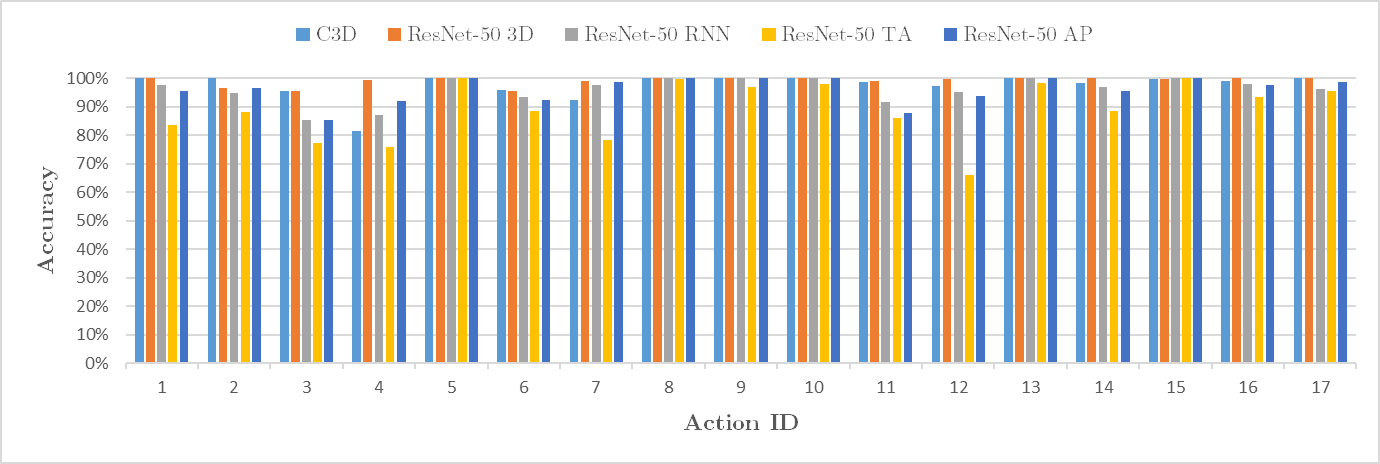
\includegraphics[width=1.0\linewidth]{figs/pc-MvDA_confusion_muhavi.png}
        \caption{Comparison of accuracy on each action class using different deep features combined with pc-MvDA.}
        %\vspace{-0.3cm}
        \label{fig:pc-MvDA_confusion_muhavi}
    \end{figure}

    Table \ref{tab:sota_muhavi} compares the best investigated combination of ResNet-50 3D and pc-MvDA with state-of-the-art frameworks. The comparison is for reference only because of aforementioned difference in setup of number of views and cross validation scheme.

    \begin{table}[htbp]
    \centering
    \caption{Comparison of the proposed methods with SOTA methods on MuHAVi dataset according to the second evaluation protocol.}
    \resizebox{0.7\textwidth}{!}{
    \begin{tabular}{|c|c|c|}
    \hline
    Methods                                                   & Cross-view & Multi-view \\ \hline
    Wu et al. \cite{wu2012view}                               & N/A       & 94.5     \\ \hline
    Zheng et al. \cite{zheng2016cross}                        & 94.88     & 99.8     \\ \hline
    Liu et al. \cite{liu2018learning}                         & N/A       & 91.2     \\ \hline
    Liu et al. \cite{liu2018hierarchically}                   & 99.91     & 99.8     \\ \hline
    Proposed method (ResNet-50 3D + pc-MvDA) \protect\footnotemark              & 99.90     & 99.88    \\ \hline
    \end{tabular}}
    \label{tab:sota_muhavi}
    \end{table}
    \footnotetext{Results when choosing only 4 views Camera 1, Camera 3, Camera 4 and Camera 6 following the other works.}
